\documentclass[11pt,a4paper]{article}

\usepackage[margin=2.45cm]{geometry}
\usepackage{microtype}
\usepackage{amsmath,amssymb}
\usepackage{booktabs}
\usepackage{graphicx}
\usepackage{xcolor}
\usepackage[hidelinks]{hyperref}

\setlength{\textfloatsep}{10pt plus 2pt minus 3pt}
\setlength{\floatsep}{8pt plus 2pt minus 2pt}
\setlength{\intextsep}{8pt plus 2pt minus 2pt}
\setlength{\abovecaptionskip}{5pt}
\setlength{\belowcaptionskip}{0pt}
\setlength{\abovedisplayskip}{6pt plus 2pt minus 2pt}
\setlength{\belowdisplayskip}{6pt plus 2pt minus 2pt}

\graphicspath{{figs/}}

\newcommand{\phivec}{\phi}
\newcommand{\xhat}{\hat{x}_{0}}
\newcommand{\abar}{\bar\alpha}

\title{Steering a nominal diffusion model\\ to synthesize spacecraft anomalies}
\author{Joon Kim \and Nils-Holger Kaul\\[0.4em]
\large DLR Galileo Competence Center}
\date{Draft, 19 October 2026}

\begin{document}
\maketitle

\begin{abstract}
\noindent
Seven years of telemetry on one spacecraft channel contain a handful of labelled
anomalies, too few to train a detector and too few to train a generator on the
anomalies themselves. We train a diffusion model on nominal operation only, and
at sampling time we steer it. Every window is edited toward a high quantile of
a soft distance to nominal reference windows. Spikes and level shifts are
additionally pinned to a sampled amplitude by an exact linear contrast, placed
at a sampled position. On the development split of ESA-ADB Mission~1, channels
41--46, the resulting windows match the height and width of the real point
anomalies, and adding them to a small detector raises event recall when real
anomalies are scarce: $+0.20$ at 32 real training windows, with a 95\% interval
that excludes zero. The same comparison is not significant once the detector
already sees every development anomaly. A prototype-pull baseline is stronger
at the smallest budgets, and an untargeted edit of the same model scores higher
on a feature-space realism metric while looking less like the requested
anomaly. Published generators on this data stay close to their nominal donors.
The sealed test split has not been opened.
\end{abstract}

\noindent\textit{This draft reports the development split only.
Section~\ref{sec:sealed} is a placeholder for a single pre-registered run on
the sealed test events.}

\section{Introduction}
\label{sec:intro}

Anomaly detection in spacecraft telemetry is limited by labels. A channel can
be recorded for years and still contain a few dozen annotated events, of
several shapes, many of which never repeat~\cite{kotowski2024esa,hundman2018lstm}.
A detector trained on those events overfits the ones it has seen. A generator
trained on them has almost nothing to fit.

The alternative is to learn the nominal process, which is abundant, and to
ask for anomalies only at sampling time. Diffusion models are a convenient
nominal model: once the denoiser is trained, a sample can be edited by changing
the predicted clean window before it is re-noised~\cite{ho2020ddpm,song2021ddim,meng2022sdedit}.
Classifier guidance and related methods already do this for images and for
time series~\cite{dhariwal2021diffusion,coletta2023guided,chung2023dps,bansal2023universal}.
What they do not supply is a target. ``Be anomalous'' is not an objective
until it is written as a function of the window.

This paper writes that function for four anomaly kinds defined by
ESA-ADB~\cite{kotowski2024esa,blazquez2021taxonomy}. Two of them, an isolated
spike and a level shift, are linear contrasts: a weighted difference of means,
with a known amplitude. The edit that realises a linear constraint in one step
is a projection, and it does not depend on the scale of the weight vector.
The other two kinds, long subsequences that sit outside the channel's usual
range or outside the range expected from their context, have no such one-line
description here. For those, and as a background term on every kind, we use a
soft distance in a frozen encoder and pull it toward a high quantile of the
same distance on nominal windows. The quantile asks for windows that are
unusual among nominal data. It does not ask for a copy of a labelled anomaly.

We evaluate the samples in two ways. The first is the realism and diversity
protocol of GenIAS~\cite{genias2025}, on a frozen twelve-dimensional feature
of each window. The second is whether the samples help a small convolutional
detector, scored by event recall at a fixed false-alarm rate, as the number of
real training anomalies varies. Both comparisons are event-held-out on the
development events. The test events stay sealed.

The result is narrower than a claim of a best generator. Against its own
unguided edit of the same donors, the contrast model is closer to real
anomalies in the frozen feature, and the morphology of its spikes and level
shifts tracks the real measurements. Against a detector trained on real
anomalies alone, the gain is concentrated at intermediate training budgets and
shrinks once real anomalies are plentiful. A cruder edit, with no contrast and
no requested shape, is closer still in the frozen feature and is the stronger
detector when data are plentiful, at the cost of spikes that collapse to one
position and a large fraction of noise bursts. We report that disagreement
rather than averaging it away. Further changes to the backbone are left as
future work; the recipe in this paper is frozen.

\section{Related work}
\label{sec:related}

Spacecraft telemetry is a poor match for detectors tuned on dense, repeated
labels. Events are rare, annotations cover an interval, and a false alarm has
an operational cost~\cite{hundman2018lstm,kotowski2024esa}. ESA-ADB is the
public form of that problem, with a shared catalogue of anomaly
types~\cite{kotowski2024esa,blazquez2021taxonomy,lai2021revisiting}. We use
that catalogue as given.

When labels are scarce, the usual synthetic anomaly is drawn by hand: a step,
a pulse, a ramp, or a change of scale~\cite{wen2021augmentation,carmona2021ncad}.
CutAddPaste pastes a real patch into another window~\cite{wang2024cutaddpaste}.
GenIAS trains a variational generator to occupy regions of a feature space
where real anomalies sit, and defines the realism and diversity scores we
report~\cite{genias2025}. All three edit an existing window. So do we. We do
not compare with generators that draw a series from pure noise.

Classifier guidance adds the gradient of a label to a diffusion
score~\cite{dhariwal2021diffusion}. Later work aims the same mechanism at
low-density regions, minority classes, and explicit time-series
constraints~\cite{sehwag2022low,um2023minority,coletta2023guided}, and applies
the correction to the clean-data prediction rather than to the
noise~\cite{chung2023dps,bansal2023universal}. SDEdit starts from a partly
noised observation so that unedited structure
survives~\cite{meng2022sdedit}; RePaint restricts that edit to a
mask~\cite{lugmayr2022repaint}. Our sampler is that SDEdit chain, with one
self-recurrence~\cite{bansal2023universal}, a causal S4 denoiser of the kind
used by TSDiff~\cite{gu2022s4,kollovieh2023tsdiff,ho2020ddpm,song2021ddim},
and a target built for these four kinds. A prototype attraction toward a real
anomaly also attracts the sample toward that anomaly's position. On ESA-ADB
the labelled window is cut with the event in the middle, so the prototype
reproduces the middle. A contrast specifies shape and amplitude and samples
the position.

\section{Data}
\label{sec:data}

We use ESA-ADB Mission~1, channels 41--46~\cite{kotowski2024esa}. Each channel
is a regularly sampled series of $7{,}364{,}160$ bins at 30\,s, which is seven
years. Windows are $W = 512$ bins, about 4.27\,hours, cut so that a labelled
event lies in the window.

The mission catalogue has 200 annotated events. We keep the benchmark split:
109 events for development and 91 for a sealed test. The test telemetry is not
read in any experiment below. Of the development events, 22 are anomalies and
the rest are rare but valid operations. Windowing the 22 anomalies gives 672
windows. Their kinds, and one real window of each, are in
Table~\ref{tab:kinds} and Figure~\ref{fig:kinds}.

\begin{table}[t]
\centering
\caption{Anomaly windows on the development split, channels 41--46. Several
windows belong to one event, so the event count is the relevant sample size
for every comparison below.}
\label{tab:kinds}
\begin{tabular}{@{}lrr@{}}
\toprule
Kind & Windows & Events \\
\midrule
Point / Global & 18 & 3 \\
Level shift & 6 & 1 \\
Global subsequence & 636 & 17 \\
Local subsequence & 12 & 2 \\
\midrule
All anomalies & 672 & 22 \\
\bottomrule
\end{tabular}
\end{table}

\begin{figure}[t]
\centering
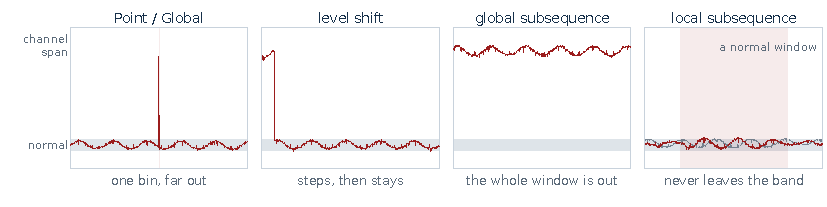
\includegraphics[width=\textwidth]{kinds.pdf}
\caption{One real anomalous window of each kind, channel~41, in channel-span
units. The grey band is the 1st to 99th percentile of nominal windows on the
same channel. A level shift and a local subsequence occupy only part of the
512 bins; the rest of the window is context.}
\label{fig:kinds}
\end{figure}

The imbalance matters. A method that only ever produced a plausible global
subsequence would already match 636 of the 672 windows and 17 of the 22
events. The level shift is a single event. Anything we report about level
shifts is a statement about that event.

The nominal training pool is 24{,}576 windows drawn from everyday operation,
plus 943 windows from the rare-but-valid events. The denoiser trains on this
pool and never sees an anomaly. A separate gallery of 1{,}536 nominal donor
windows, 256 per channel, is the starting point for every generated sample.
Development anomalies are partitioned into three folds by event, with 270, 276
and 126 windows. A fold's test events are never used to choose that fold's
contrast amplitudes, except for the level shift on the fold that contains its
only event, which is discussed in Section~\ref{sec:limits}.

\section{Method}
\label{sec:method}

\subsection{Nominal diffusion model}

Each window is scaled to $[0, 1]$ by a per-channel minimum and maximum fit on
the nominal training pool, and the denoiser is trained in that space. The
forward process has $T = 200$ steps with a linear noise schedule from
$\beta = 10^{-4}$ to $\beta = 2 \cdot 10^{-2}$~\cite{ho2020ddpm}. The network
predicts the added noise. It is an S4 model with hidden width 64, six layers
and state size 64, causal, conditioned on the channel index
\cite{gu2022s4,kollovieh2023tsdiff}. Training is 20{,}000 steps of noise-prediction
loss, batch size 128, learning rate $2 \cdot 10^{-4}$, on the 24{,}576 nominal
windows and 943 rare windows. The network has $315{,}841$ parameters. Anomalies
are not in this training set.

The network is causal, so a bin is denoised without seeing the future. At
sampling time we evaluate it twice and blend the noise predictions,
\begin{equation}
\label{eq:flip}
\varepsilon(x)_{i}
  = r_{i}\,\varepsilon_{\theta}(x)_{i}
  + (1 - r_{i})\,
    \bigl(\varepsilon_{\theta}(\mathrm{flip}\, x)\bigr)_{\!\mathrm{flip},\, i},
\qquad
r_{i} = \frac{i}{L - 1}.
\end{equation}
The second pass is the same network reading the window backwards. The ramp
gives it the start of the window and gives the forward pass the end. The
weights are unchanged. We do not train a bidirectional backbone.

\subsection{Where an edit starts}

Generation starts from a nominal donor, not from pure noise. The donor is
noised to time index
\begin{equation}
\label{eq:t0}
t_{0} = \mathrm{round}\bigl(0.2 \cdot (T - 1)\bigr) = 40
\end{equation}
and then denoised with 50 DDIM steps from $t_{0}$ down to $0$
\cite{song2021ddim,meng2022sdedit}. The next state is the ordinary DDIM step
on an edited clean window,
\begin{equation}
\label{eq:ddim}
x_{t'}
  = \sqrt{\abar_{t'}}\,(\xhat - E)
  + \sqrt{1 - \abar_{t'}}\,\varepsilon(x_{t}).
\end{equation}
$E$ has the same length as the window. It is a shell term, on every kind, plus
a contrast term on spikes and level shifts only. After each step that
advances, the result is re-noised to $t$ and the step is run once
more~\cite{bansal2023universal}. On the final step $E$ is multiplied by $1/4$.

The shell term is multiplied along the chain by a weight proportional to the
remaining noise $\sigma_{t} = \sqrt{(1 - \abar_{t})/\abar_{t}}$, renormalized
so that the weights average to one. Early steps, which still have noise left
to remove, carry more of the shell edit than late steps. The contrast term is
not decayed.

\subsection{Shell term}

Let $e(\cdot)$ be a frozen convolutional encoder and $r_{1}, \ldots, r_{N}$ a
set of $N = 512$ nominal reference embeddings. The soft energy of an embedding
$z$ is
\begin{equation}
\label{eq:h}
h(z)
  = -\tau \log \sum_{j=1}^{N}
    \exp\bigl(-\lVert z - r_{j}\rVert^{2} / \tau\bigr),
\end{equation}
a soft minimum of squared distance to the references. As $\tau \to 0$ it
becomes the distance to the nearest reference. Large $h$ means far from every
nominal reference. Because of the $-\tau \log N$ contribution of the sum, $h$
is not itself a distance and need not be positive.

The encoder keeps the time axis. Three stride-2 convolutions
($1 \to 32$, kernel 7; $32 \to 64$, kernel 5; $64 \to 64$, kernel 5), each
followed by a SiLU, reduce 512 bins to 64, and a pointwise convolution maps
the 64 channels to 8. The embedding is the resulting $8 \times 64$ map, flattened
to 512 dimensions. It is trained with a reconstruction loss and a supervised
contrastive loss~\cite{khosla2020supcon} on three classes: everyday nominal,
rare-but-valid, and anomaly. The checkpoint used for every fold is the one
trained when fold~0 is held out, so its anomaly class is the anomalies of
folds~1 and~2. Section~\ref{sec:limits} records what that implies.

Let $Q$ be the 0.99 quantile of $h$ on held-out nominal windows. The one
percent of nominal windows above $Q$ are the most unusual nominal windows, so
$Q$ is the upper edge of ordinary operation, not a typical value. The shell
loss on a predicted clean window is the squared distance of its energy to that
edge, $(h - Q)^{2}$, averaged over the batch. The shell edit is $\lambda = 0.3$
times the gradient of this loss with respect to $\xhat$, divided by the
gradient's Euclidean norm. Subtracting it, as in~\eqref{eq:ddim}, moves $h$
toward $Q$. The same term runs on all four kinds. It is the only term on the
two subsequence kinds.

\subsection{Contrast term}

A spike and a level shift are each specified by a linear functional
$d(x) = \langle w, x \rangle$ and a target amplitude $a$. The weight $w \in
\mathbb{R}^{512}$ sums to zero, so $d$ is blind to the window's overall level.

For a spike at bin $p$, with the half-width set to zero, $w$ equals $+1$ at
$p$. It equals $-1/m$ on the flanking bins that remain after a gap of three
bins, up to eight bins on each side, and $m$ is the number of those flank bins.
Then $d(x)$ is the height of the centre bin above the mean of its flanks.
For a level shift whose high side is the head of the window and whose split is
at $p$, $w$ equals $+1/p$ on the head and $-1/(W - p)$ on the tail, so $d(x)$
is the difference between the two means. Reversing $w$ moves the high side to
the tail without changing the amplitude.

The edit that realises $\langle w, \xhat - E \rangle = a$ and changes $\xhat$
as little as possible in Euclidean norm is the projection
\begin{equation}
\label{eq:contrast}
E_{\mathrm{contrast}}
  = \bigl(\langle w, \xhat \rangle - a\bigr)\,
    \frac{w}{\lVert w \rVert^{2}}.
\end{equation}
It is an exact solution, not a gradient step of a fixed size, and it is
unchanged if $w$ is multiplied by a constant. We add it to the shell edit.
The implementation subtracts $E$ inside~\eqref{eq:ddim}, so a window whose
contrast is already $a$ is left unchanged by this term.

Three quantities are sampled per window, and they are the freedom in the
contrast. The position is uniform on the bins where $w$ is defined. For a
level shift the split is drawn from $6.25\%$ to $18\%$ of the window, which
is the range of the real event, and the weight is reversed with probability
$1/2$, so the step is not always at the same end. The amplitude $a$ is drawn
from the values of $d$ measured on real windows of that kind outside the query
fold. If the requested sign would push the donor outside the channel span
$[0, 1]$ and the opposite sign would not, the sign is flipped and the
magnitude is kept. After the guided chain, a level shift is re-noised to
$35\%$ of the schedule and denoised for ten steps with $E = 0$, and the
contrast is then applied once more. That pass is an SDEdit polish
\cite{meng2022sdedit}: it asks the nominal denoiser to rebuild the texture
around a step that the polish would otherwise shrink.

The two subsequence kinds have no contrast. They receive the shell edit only.
Dropping the contrast, rather than adding a prototype attraction toward a real
anomaly embedding, is deliberate. A prototype of a centred event teaches the
centre.

There is no spatial mask. An earlier variant replaced every bin outside a mask
with the noised donor at each step, as in RePaint~\cite{lugmayr2022repaint},
and could export the mask as a bin-level label. Removing the mask lets the
chain rewrite the whole window. Section~\ref{sec:results} compares the two.

Donors are assigned to kinds inside each channel, in equal counts, so each
kind is generated on every channel. A gallery of 1{,}536 donors therefore
contains 384 windows of each kind. The real window counts in
Table~\ref{tab:kinds} are not equal, and the generated training data do not
pretend that they are.

\begin{figure}[t]
\centering
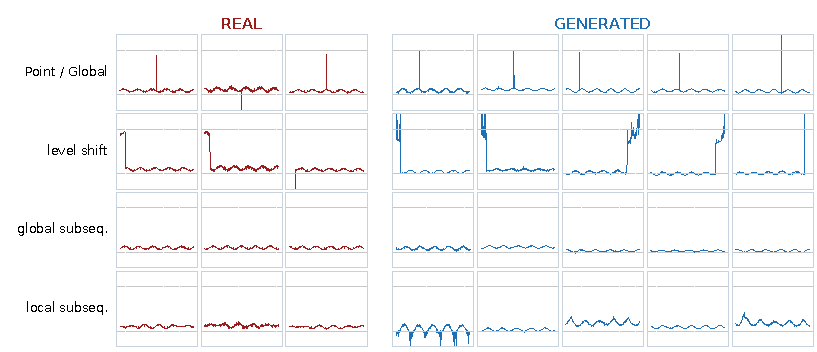
\includegraphics[width=\textwidth]{gallery.pdf}
\caption{Three real windows and five generated windows of each kind, in
channel-span units. Generated windows are from the contrast model. Dotted
lines are the channel span, 0 and 1.}
\label{fig:gallery}
\end{figure}

\section{Evaluation}
\label{sec:eval}

\subsection{Realism and diversity}

Following GenIAS~\cite{genias2025}, each window is mapped to a frozen feature
$\phivec \in \mathbb{R}^{12}$: the mean, standard deviation, minimum and
maximum of the window after it has been z-scored, the mean and standard
deviation of its first difference, its peak absolute value, the longest run of
bins whose absolute z-score exceeds one, and the log-energy of four Fourier
bands. No coefficient of $\phivec$ is trained, and $\phivec$ is not the
encoder used for steering.

Let $A$ be the real anomalous windows of a query fold and $G$ a generated
gallery. With $d(a) = \min_{g \in G} \lVert \phivec(a) - \phivec(g)\rVert_{2}$,
\begin{equation}
\label{eq:arp}
\mathrm{ARP}
  = \frac{1}{1 + \lvert A\rvert^{-1}\sum_{a \in A} d(a)}.
\end{equation}
ARP is high when real anomalies lie close to some generated window. It says
nothing about whether the rest of the gallery is far away, and nothing about
which kind was requested. Coverage at a frozen radius $\tau = 0.105$ is the
fraction of $a \in A$ with $d(a) \le \tau$. The radius was set so that an
unguided full-noise gallery covers about ten percent of real anomalies, and
it is not retuned.

Diversity has two summaries. The mean pairwise distance in $\phivec$ is
scale-dependent and unbounded. The entropy diversity index partitions the
union of the real query windows and every gallery in the comparison by
$k$-means with $k = 16$, seed 0, and reports the Shannon entropy of each
gallery's share of those regions. The ceiling is $\log 16 \approx 2.77$. The
partition depends on which galleries are included, so the entropies in
Table~\ref{tab:realism} are comparable to each other and not to an entropy
computed on a different set of methods. We refit the partition on each fold
and average.

A classifier two-sample test asks whether real anomalies and generated windows
can be told apart~\cite{lopezpaz2017c2st}. We report two versions, because
they disagree. One is a logistic regression on $\phivec$, the other a ridge
classifier on ROCKET features of the raw window~\cite{dempster2020rocket}.
Both are grouped so that windows of one event do not sit on both sides of a
split. An area of $1/2$ means the classifier is at chance.

Three galleries anchor the scale of ARP. Real anomalies from the training
folds, offered as a gallery, score 0.792. The nominal donors score 0.320.
White noise scores 0.158. A generated gallery that does no more than copy its
donor lands near 0.32, whatever its diagrams look like.

\subsection{Does the gallery help a detector?}

The detector is a small convolutional network: three stride-2 convolutions
($1 \to 32$, kernel 7; $32 \to 64$, kernel 5; $64 \to 64$, kernel 5) with
SiLU nonlinearities, global average pooling, and a linear map to one logit.
It has 31{,}169 parameters. It is trained with balanced batches of anomalies
against nominal and rare windows, binary cross-entropy, Adam at learning rate
$10^{-3}$, for 400 steps. The decision threshold is the empirical 1\%
false-alarm point on held-out nominal windows. An event is counted as found if
any of its windows exceeds the threshold. The reported number is event recall,
the fraction of the 22 development events that are found.

Two operating points are easy to confuse. At the full budget the detector
sees every training-fold anomaly window, on the order of four hundred, plus
256 generated windows. At budget $k$ it sees $k$ real anomaly windows plus $k$
generated ones. The real subset is drawn once per fold and seed and shared by
every method, so differences are paired. We use five seeds and the three event
folds. Paired differences are bootstrapped over the 22 events
\cite{efron1994bootstrap}. With 22 events the intervals are wide; a difference
whose interval contains zero is reported as unresolved, including when the
bootstrap tail probability is just under 0.05.

The generated gallery for a fold is built without that fold's anomaly events,
with the level-shift exception already noted. Published and hand-built
baselines are given the same donors: a locked GenIAS checkpoint, a
reimplementation of the published GenIAS procedure, CutAddPaste
\cite{wang2024cutaddpaste}, and a hand-built injector that adds a step, pulse,
ramp or scale change of random amplitude. The reimplemented GenIAS differs
from its donor by an RMSE of $2.3 \cdot 10^{-3}$ in channel-span units.

\subsection{Ablations of the edit}

Four variants share the denoiser, the donors, the schedule and the seeds.
The \emph{contrast model} is the method above. The \emph{masked} variant is
the same method with the RePaint mask restored. The \emph{shell-only} variant
applies the shell edit and no contrast, so it never asks for a spike or a step.
The \emph{twin} is the same chain with every edit turned off: a partly noised
donor, denoised, and nothing else. The \emph{prototype} baseline replaces the
contrast with an attraction in the encoder toward the embedding of a real
anomaly of the assigned kind, which is the natural use of the labelled windows
and the one that inherits their positions.

\section{Results}
\label{sec:results}

\subsection{What the windows look like}

Figure~\ref{fig:gallery} shows real and generated windows. The numerical
counterpart is Table~\ref{tab:morph}. Spike height and the share of spikes
that occupy a single bin are measured in channel-span units. The contrast
model lands on the real spike (height 0.838 against 0.831, 99\% of draws a
single bin). The masked variant, which was built to protect the baseline,
overshoots the height and spreads a third of the spikes over more than one
bin. The prototype and the shell-only edit produce spikes of about half the
real height, and about 22\% of their point-anomaly draws are noise bursts
rather than spikes. The contrast model still produces a noise burst in 3\% of
draws. More visibly, 14.8\% of its point-anomaly draws contain three or more
deep downward dips in the baseline. The real windows have none. The mask
suppresses these dips, because it holds the baseline at the donor, and the
prototype is worse (48\%).

Level shifts from the contrast model are 1.21 times as rough as the real
event, against 1.53 times for the masked variant. The baseline texture around
its spikes is 0.83 times the real texture, so the window is slightly smoother
than the data. The edit touches 42\% of bins in a typical window and 29\% of
bins in a point anomaly. The masked variant touches under 1\% of a point
anomaly, which is the spike itself, and therefore has a bin-level label. The
contrast model does not.

\begin{table}[t]
\centering
\caption{Morphology of point anomalies and level shifts, development
galleries. Spike height is in channel-span units. Roughness and texture are
ratios to the real windows. A noise burst is a point-anomaly draw whose
baseline is more than three times the real baseline texture. Deep dips are
point-anomaly draws with three or more large downward spikes beside the
requested one.}
\label{tab:morph}
\setlength{\tabcolsep}{4.5pt}
\small
\begin{tabular}{@{}lrrrrr@{}}
\toprule
 & Real & Contrast & Masked & Shell only & Prototype \\
\midrule
Spike height & 0.831 & 0.838 & 0.988 & 0.496 & 0.447 \\
Single-bin spikes & 100\% & 99\% & 53\% & 85\% & 53\% \\
Noise bursts & 0\% & 3.0\% & 0\% & 22\% & 23\% \\
Deep dips ($\ge 3$) & 0\% & 14.8\% & 2.0\% & --- & 48\% \\
Level-shift roughness & 1 & 1.21$\times$ & 1.53$\times$ & 1.58$\times$ & 1.70$\times$ \\
Baseline texture & 1 & 0.83$\times$ & 0.97$\times$ & 1.08$\times$ & 2.00$\times$ \\
\bottomrule
\end{tabular}
\end{table}

\subsection{Feature-space realism}

Table~\ref{tab:realism} is the GenIAS protocol. The contrast model reaches ARP
0.509, against 0.318 for its twin and about 0.32 for every published or
hand-built editor, which sit on the donor. The GenIAS reimplementation is
slightly below the donor, consistent with its RMSE. Relative to the anchors,
0.509 lies between the donor (0.320) and an oracle gallery of real anomalies
(0.792). It is not the best ARP in the table: the shell-only edit scores
0.579 and the prototype 0.567.

The paired ARP gain over the twin averages $+0.191$, interval
$[+0.039, +0.346]$, from fold-wise gains $+0.143$, $+0.051$ and $+0.381$.
Standardizing $\phivec$ shrinks those three numbers to $+0.025$, $+0.005$ and
$+0.202$. Coverage moves the other way, from 8.1\% for the twin to 3.8\% for
the contrast model: average distance falls, and so does the fraction of real
anomalies inside the protocol's ball. The misses are mostly global
subsequences, which dominate $A$ and which the contrast does not build.
Entropy is 2.33 for the contrast gallery and 1.06 for the real anomalies in
the same partition, so the gallery spreads into regions the real set does not
occupy. Pairwise distance is 10.5 against 1.7 for the twin and about 1.1 for
the editors.

The two classifier tests disagree with ARP and with each other. On
$\phivec$, logistic regression separates the contrast gallery from real
anomalies at AUC 0.645, the prototype at 0.662 and the twin at 0.517, so by
this test steering makes a sample easier to reject. On ROCKET features the
twin is rejected at 0.905, the contrast model at 0.880, the shell-only edit
at 0.882 and the prototype at 0.966. Neither AUC is the objective the sampler
maximises.

\begin{table}[t]
\centering
\caption{Realism on the development folds. ARP, coverage and pairwise
distance are means over the three event folds. Entropy is the mean of three
partitions, each fit to that fold's real anomalies together with every gallery
listed here ($k = 16$, seed 0). The real row has no ARP: it would be the
distance from a set to itself.}
\label{tab:realism}
\small
\begin{tabular}{@{}lrrrr@{}}
\toprule
Gallery & ARP & Cov. & Entropy & Pairwise \\
\midrule
Real anomalies & --- & --- & 1.06 & --- \\
Contrast (ours) & 0.509 & 0.038 & 2.33 & 10.53 \\
Contrast, masked & 0.499 & 0.033 & 2.32 & 9.68 \\
Shell only & 0.579 & 0.029 & 2.37 & 8.83 \\
Prototype & 0.567 & 0.015 & 2.34 & 7.30 \\
Twin (no edit) & 0.318 & 0.081 & 0.97 & 1.71 \\
\midrule
GenIAS, locked & 0.317 & 0.195 & 0.72 & 1.09 \\
GenIAS, reimplemented & 0.290 & 0.053 & 0.17 & 0.80 \\
CutAddPaste & 0.322 & 0.290 & 0.72 & 1.11 \\
Hand-built shapes & 0.319 & 0.267 & 0.74 & 1.21 \\
Nominal donor & 0.320 & 0.354 & 0.71 & 1.11 \\
\bottomrule
\end{tabular}
\end{table}

\subsection{Event recall}
\label{sec:detect}

At the full budget, with every training-fold anomaly available, median event
recall is 0.591 for real anomalies alone and 0.682 with the contrast gallery
added (mean 0.655, average precision 0.485, window AUROC 0.617). The paired
difference is $+0.091$ with interval $[-0.045, +0.236]$. The interval contains
zero. GenIAS, the reimplementation and CutAddPaste all sit at median 0.545,
below real data alone (GenIAS minus real data is $-0.027$, interval
$[-0.055, 0]$). The hand-built shapes match real data at 0.591. The contrast
model's false-alarm rate on rare-but-valid events rises from 0.026 to 0.059,
so part of the recall is paid for in alarms on operations that are unusual and
not anomalous.

The shell-only edit, in the same detector protocol, reaches median recall
0.727, and the prototype reaches 0.636. The ordering at the full budget is
the ordering of ARP, not the ordering of spike morphology. A window-level
network can use a large, unstructured deviation. It does not need the
deviation to be a one-bin spike.

Figure~\ref{fig:sweep} and Table~\ref{tab:sweep} are the comparison the
generator is for: $k$ real anomaly windows, plus $k$ generated ones. For the
contrast model the 95\% interval excludes zero at $k = 8$, $32$ and $64$
($+0.155$, $+0.200$, $+0.136$), and the $k = 32$ interval is
$[+0.073, +0.318]$. At $k \le 4$ and from $k = 128$ up, the interval contains
zero, and the prototype is ahead at the small end. Putting the prototype
attraction back on top of the contrast changes the $k = 32$ gain from
$+0.200$ to $+0.182$. Restoring the mask cuts it to $+0.109$. The twin does
not help. The annotation in Figure~\ref{fig:sweep} is that paired $+0.200$,
not the vertical gap between the two median curves.

Rank-fusing the detector logit with a label-free diffusion reconstruction
score changes the full-budget comparison: the contrast model minus real data
becomes $+0.136$ with interval $[+0.036, +0.264]$. That is a different system.
We do not use it as the primary endpoint.

\begin{figure}[t]
\centering
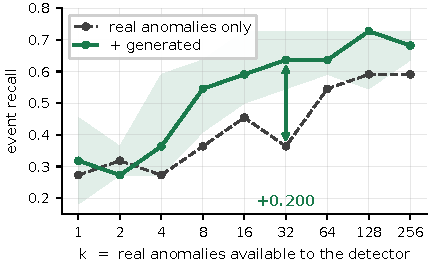
\includegraphics[width=0.64\textwidth]{sweep.pdf}
\caption{Event recall of a detector trained on $k$ real anomaly windows (dashed)
or on those windows plus $k$ windows from the contrast model (solid). The band
is the minimum and maximum over five seeds. The annotation at $k = 32$ is the
paired difference $+0.200$, not the gap between the plotted medians.}
\label{fig:sweep}
\end{figure}

\begin{table}[t]
\centering
\caption{Paired change in event recall relative to the same $k$ real windows
and no synthetic windows. Five seeds, three folds, bootstrap over 22 events.
An interval that excludes zero is marked. Medians can tie while paired
differences differ, because the pairing is at the level of events.}
\label{tab:sweep}
\small
\begin{tabular}{@{}rrrrrrr@{}}
\toprule
 & \multicolumn{2}{c}{Contrast} & \multicolumn{2}{c}{Prototype} & \multicolumn{2}{c}{Shell only} \\
\cmidrule(lr){2-3}\cmidrule(lr){4-5}\cmidrule(lr){6-7}
$k$ & median & $\Delta$ & median & $\Delta$ & median & $\Delta$ \\
\midrule
1  & 0.318 & $+0.01$ & 0.409 & $+0.09$ & 0.318 & $+0.04$ \\
8  & 0.545 & $+0.15^{\ast}$ & 0.545 & $+0.18^{\ast}$ & 0.500 & $+0.10^{\ast}$ \\
32 & 0.636 & $+0.20^{\ast}$ & 0.636 & $+0.24^{\ast}$ & 0.591 & $+0.16^{\ast}$ \\
64 & 0.636 & $+0.14^{\ast}$ & 0.636 & $+0.13^{\ast}$ & 0.636 & $+0.10$ \\
256 & 0.682 & $+0.11$ & 0.636 & $+0.08$ & 0.727 & $+0.12$ \\
\bottomrule
\end{tabular}\\[0.3em]
{\footnotesize $^{\ast}$95\% bootstrap interval excludes zero.
Real-only medians at these $k$ are 0.273, 0.364, 0.364, 0.545, 0.591.}
\end{table}

\subsection{Held-out test}
\label{sec:sealed}

The 91 test events have not been used. The pre-registered test report is one
run of the contrast model, with the frozen $\phivec$ and the same detector, at
full budget and at $k = 32$, with no retuning after the numbers are seen.
Until that run, every claim above is a claim about the 22 development events.

\section{Limitations}
\label{sec:limits}

Every interval in this paper is computed on 22 events, and the level-shift
numbers are one event. The three fold-wise ARP gains are $+0.143$, $+0.051$
and $+0.381$.

Global and local subsequences are steered only by the shell. On this split
the shell energy ranks labelled anomalies against nominal windows at an AUROC
of about 0.54, so $Q$ means unusual among nominal windows, not similar to a
labelled subsequence. Those two kinds are 648 of the 672 windows. A budget
sweep that draws real windows uniformly is mostly a sweep over subsequences;
a kind-stratified sweep is not here. The steering encoder is the fold-0
checkpoint on every fold, and its contrastive loss was trained on the
anomalies of folds~1 and~2, so the shell gradient for those folds is taken in
a representation that has seen their labels. The contrast term does not use
the encoder. The subsequence windows have no contrast, so they do. All six
level-shift windows are one event in one fold: the other folds borrow its
amplitude, and its own fold measures the amplitude on itself.

A quarter of each gallery is each kind, against 95\% global subsequences in
the real windows. The kind assignment alone does not explain the detector
gain, because the twin uses it and does not help, but the gallery is still
not the mission's prior. The shell-only edit wins ARP and full-budget recall
without placing the spike it was not asked for; the contrast model does the
reverse. Bin-level localisation, where a known position should matter, is not
implemented. The masked model is the one with a mask, and it is the weaker
detector. Beating GenIAS, CutAddPaste and the hand-built shapes is a weak
claim on these donors: they remain within a few thousandths of the donor in
RMSE, and their ARP is the donor's. The comparisons that carry weight are the
twin, the prototype, the shell-only edit, and real data alone.

The denoiser stays causal apart from~\eqref{eq:flip}, the schedule stays
linear, and samples start from a donor at $t_{0} = 40$. Other channels and
other missions are untouched. None of those changes would repair a missing
subsequence target or an interval computed on 22 events.

\section{Conclusion}

A nominal diffusion model can be steered into spikes and level shifts whose
size matches the few labelled examples, by a shell quantile plus an exact
linear contrast. On the development events of ESA-ADB Mission~1, channels
41--46, the windows help a small detector when real anomalies number in the
tens, and the gain is unresolved once every development anomaly is already
available. A prototype baseline leads at the smallest budgets. An untargeted
shell edit leads on feature-space realism and on full-budget recall, and about
one point-anomaly draw in seven still carries a run of deep baseline dips. We
stop at this recipe. Subsequence targets, a bin-level detector, a
kind-stratified budget, and one pre-registered run on the sealed test are the
open measurements. A bidirectional backbone, a different noise schedule, and
sampling from pure noise are future work, not a requirement for reporting
what this recipe does.

\bibliographystyle{plain}
\bibliography{refs}

\end{document}
